\documentclass[../differential_methods.tex]{subfiles}
\begin{document}
\section{Aula 10 - 15 de Abril, 2026}
\subsection{Motivações}
\begin{itemize}
	\item Métodos Preditor-Corretor
\end{itemize}
\subsection{Métodos do tipo Preditor-Corretor}
Esse tipo de método é uma estratégia para utilizar métodos implícitos sem recorrer ao método de Newton. Por isso, considere o seguinte método implícito:
\[
	\mathbf{U}^{n+1} = \mathbf{U}^{n} + h \varphi_{c}(\mathbf{U}^{n+1}, \mathbf{U}, t_{n}, h);
\]
pode-se definir um processo iterativo para determinar \(\mathbf{U}^{n+1}\), como por exemplo
\[
	\mathbf{U}^{n+1, [s+1]} = \mathbf{U}^{n} + h \varphi_{c}(\mathbf{U}^{n+1, [s]}, \mathbf{U}^{n}, t_{n}, h), \quad s=0, 1, 2, \dotsc , m-1.
\]
O valor inicial desse processo iterativo pode ser obtido por um método explícito da forma
\[
	\mathbf{U}^{n+1, [0]} = \mathbf{U}^{n} + h \varphi_{p}(\mathbf{U}^{n}, t_{n}, h).
\]
Neste contexto, o método definidor por \(\varphi_{p}\) é chamado \textbf{preditor}, e o método definido por \(\varphi_{c}\) é o \textbf{corretor}, e o processo total é conhecido como \textbf{método preditor-corretor}, especificamente \(PC^{m}\).

\begin{example}[Euler-Trapézio]

	Considere o método preditor \(\varphi_{p}\) como sendo, por exemplo, o método de Euler, e o corretor como sendo o método do trapézio; neste caso, o método preditor-corretor \(PC^{m}\) é dado por
	\begin{align*}
		 & \mathbf{U}^{n+1, [0]} = \mathbf{U}^{n} + h \mathbf{f}(\mathbf{U}^{n}, t_{n})                                                                                   \\
		 & \mathbf{U}^{n+1, [s+1]} = \mathbf{U}^{n}+ \frac{h}{2}(\mathbf{f}(\mathbf{U}^{n+1, [s]}, t_{n+1}) + \mathbf{f}(\mathbf{U}^{n}, t_{n})), \; s = 0, \dotsc , m=1.
	\end{align*}
\end{example}

A convergência desse método ocorre se existe uma jacobiana \(J_{G}\) com norma \(\Vert J_{G} \Vert \leq \mathcal{J}< 1\), pois, neste caso,
\[
	\Vert x^{k+1}-x^{k} \Vert \leq \mathcal{J}\Vert x^{k}-x^{k} \Vert.
\]

Existe um teorema nos dá um estimativa do número de iterações necessárias para atingir a ordem máxima de convergência, e qual ela é:

\begin{theorem*}
	Seja p a ordem de consistência do método preditor e q a ordem do método corretor; então, o método preditor-corretor \(PC^{m}\) tem ordem de conssitência \(\mathcal{O}(h^{\min\limits_{}(q, p+m)})\).
\end{theorem*}

Em termos de precisão, ele não diz muita coisa, mas não adiantam muitas iterações, pois o erro geral do método é limitado pelo erro de truncamento, que, por sua vez, depende de potências de h; o mesmo vale quando se utiliza diretamente do método de Newton para o problema não linear!
Uma boa coisa desse método é para fazer predições temporais!

\begin{example}[Preditor-Corretor para Lotka-Volterra]
	O preditor aqui é o método de Euler explícito, dado por
	\[
		\begin{bmatrix}
			U_{1}^{n+1, [0]} \\
			U_{2}^{n+1, [0]}
		\end{bmatrix} = \begin{bmatrix}
			U_{1}^{n} \\
			U_{2}^{n}
		\end{bmatrix} + h \begin{bmatrix}
			-2U_{1}^{n} + U_{1}^{n}U_{2}^{n} \\
			U_{2}^{n} - U_{1}^{n} U_{2}^{n}
		\end{bmatrix},
	\]
	e o corretor seria o trapézio
	\[
		\begin{bmatrix}
			U_{1}^{n+1, [s+1]} \\
			U_{2}^{n+1, [s+1]}
		\end{bmatrix} = \begin{bmatrix}
			U_{1}^{n} + \frac{h}{2}\biggl(\begin{bmatrix}
					                              -2U_{1}^{n+1, [s]} + U_{1}^{n+1, [s]} U_{2}^{n+1, [s]} \\
					                              U_{2}^{n+1, [s]} - U_{1}^{n+1, [s]}U_{2}^{n+1, [s]}
				                              \end{bmatrix} + \begin{bmatrix}
					                                              -2U_{1}^{n } + U_{1}^{n}U_{2}^{n} \\
					                                              U_{2}^{n} - U_{1}^{n} U_{2}^{n}
				                                              \end{bmatrix}\biggr).
		\end{bmatrix}
	\]

	Implementado como código, temos
	\begin{listing}[H]
		\caption{Implementação Preditor-Corretor de Lotka-Volterra}
		\begin{minted}[bgcolor = bg, linenos=true, breaklines]{Matlab}
       function fd = f_pp ( u)

       fd (1 ,1) = -2* u (1) + u (1) *u (2) ;
       fd (1 ,2) = u (2) - u (1) * u (2) ;

      ...
      while tn < tfim

        fn = f_pp ( un ) ;

        % Preditor Euler explicito
        un1 = un + h * fn (1 ,:) ;

        % Corretor trapezio
        for i =1: M
          fn1 = f_pp ( un1 );
          un1 = un + 0.5* h *( fn (1 ,:) + fn1 (1 ,:) ) ;
        end

        tn = tn + h;
        un = un1 ;

      end
      ...
     \end{minted}
	\end{listing}
	O gráfico resultante é
	\begin{figure}[H]
		\begin{center}
			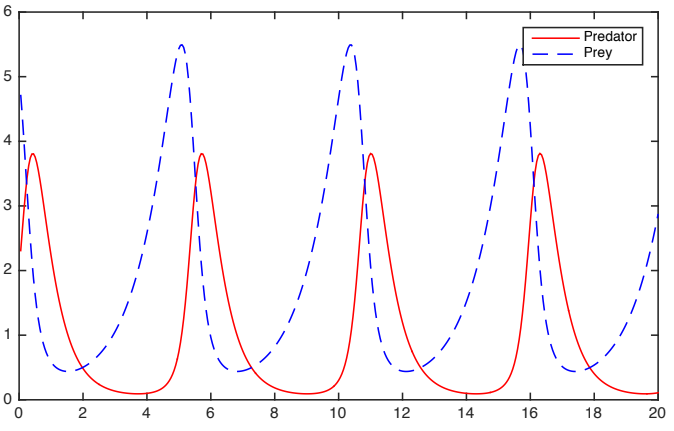
\includegraphics[height=0.8\textheight, width=0.8\textwidth, keepaspectratio]{./Images/predictor_corrector_10.png}
		\end{center}
		\caption{comparação da população da presa com a do predador}
	\end{figure}

\end{example}

As imagens de cada um dos métodos ajudam bem a ver como eles se comparam:

\begin{figure}[H]
	\begin{center}
		\caption{erros de diferentes métodos nas próximas imagens}
		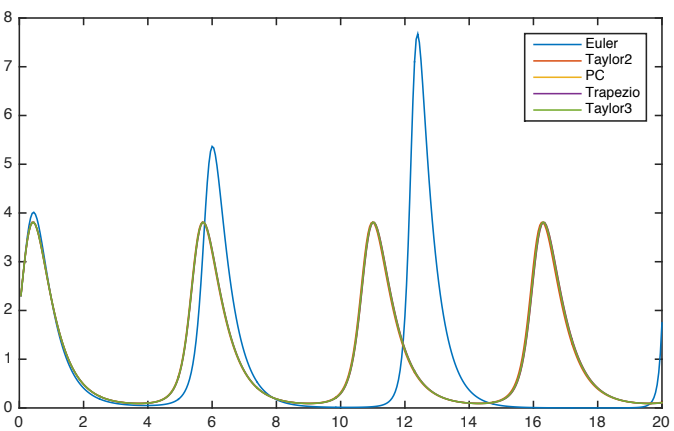
\includegraphics[height=0.8\textheight, width=0.8\textwidth, keepaspectratio]{./Images/methods_10.png}
	\end{center}
\end{figure}
\begin{figure}[H]
	\begin{center}
		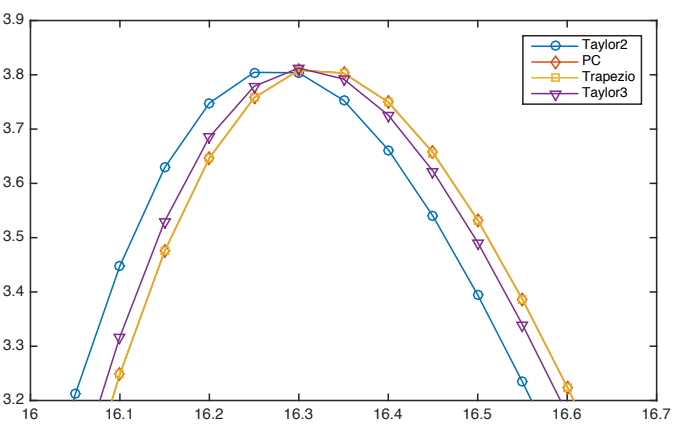
\includegraphics[height=0.8\textheight, width=0.8\textwidth, keepaspectratio]{./Images/implicits_10.png}
	\end{center}
\end{figure}

E é interessante comparar os erros do método de Newton com o \(PC^{m}\) para lidar com implícitos.
\begin{figure}[H]
	\begin{center}
		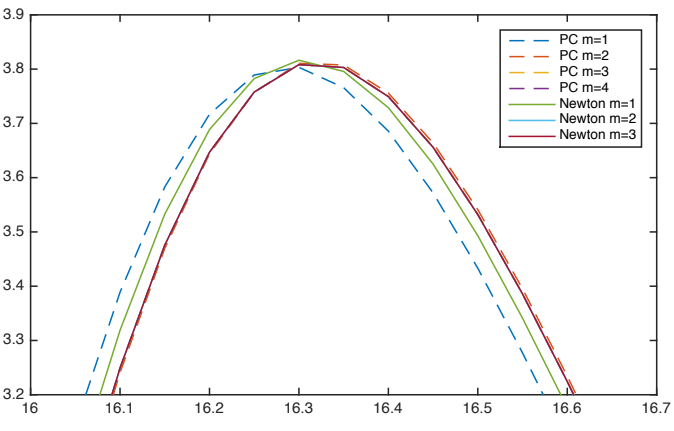
\includegraphics[height=0.8\textheight, width=0.8\textwidth, keepaspectratio]{./Images/newton_pcm_10.png}
	\end{center}
\end{figure}

No fim, fica a pergunta: por que usar os métodos implícitos, se eles são mais difíceis de serem calculados? Vamos ver um exemplo que responda isso.

Considere um problema linear da forma
\[
	u'(t) = -\lambda u(t),\; u(0)=1
\]
com \(\lambda > 0\), cuja solução exata é \(u(t) = e^{-\lambda t}\), de modo que
\[
	\lim_{t\to \infty}u(t) = 0.
\]
O método de Euler explícito para esse caso simples fica
\begin{align*}
	U^{n+1} = U^{n}-h\lambda U^{m} = (1-h\lambda ) U ^{n} & = (1-h\lambda )^{2}U^{n-1} \\
	                                                      & \vdots                     \\
	                                                      & = (1-h\lambda )^{n}U^{0},
\end{align*}
tal que a solução aproximada satisfaz
\[
	\lim_{n\to \infty}U^{n} = 0 \Longleftrightarrow | 1-h\lambda  |<1.
\]

O problema disso é que acaba impondo uma restrição sobre a escolha do passo h, que, caso não seja satisfeita, pode produzir soluções desastrosas nas quais \(U^{n}\) diverge ao infinito! No caso do método de Euler explícito, a restrição é
\[
	h < \frac{2}{\lambda }.
\]

Por outro lado, vamos replicar as ideias acima para um método implícito, digamos o trapézio; nele, tem-se
\[
	U^{n+1} = U^{n} - \frac{h}{2}(\lambda U^{n} + \lambda U^{n+1}) \Rightarrow U^{n+1} = \biggl(\frac{1-\frac{h\lambda }{2}}{1+\frac{\lambda h}{2}}\biggr)^{n}U^{0},
\]
donde concluímos que, independente da escolha de h, teremos \(\lim_{n\to \infty}U^{n}=0\) -- métodos implícitos são mais robustos! O mesmo acontece até para o método de Euler implícito.

\subsection{Estabilidade Absoluta}
Consideremos um problema escalar linear da forma
\[
	u'(t) = \lambda u(t),\; u(0) = \lambda ,\quad \lambda \in \mathbb{C},
\]
cuja solução é da forma
\[
	u(t) = \lambda e^{\lambda t} = \lambda e^{(\mathrm{Re}(\lambda ) + i \mathrm{Im}(\lambda ))t} \Rightarrow | u(t) | = \lambda e^{\mathrm{Re}(\lambda )t},
\]
onde \(\mathrm{Re}(\cdot )\) e \(\mathrm{Im}(\cdot )\) denotam, respectivamente, as partes reais e imaginárias da expressão. Com isso, temos alguns casos relacionados ao crescimento da solução:

\begin{itemize}
	\item[\(\mathrm{Re}(\lambda )>0\):] aqui, a solução \(| u(t) |\) cresce exponencialmente com t, tornando-se \textit{instável};
	\item[\(\mathrm{Re}(\lambda )=0\):] neste caso, a solução é \(| u(t) | = \lambda \), e ela fica oscilando;
	\item[\(\mathrm{Re}(\lambda )<0\):] finalmente, \(| u(t) |\) decai exponencialmente com t, sendo \textit{estável}.
\end{itemize}
O caso que mais nos interessa inicialmente é a estabilidade do método numérico, então analisaremos este último caso.

\begin{def*}
	Um método geral de um passo é dito \textbf{absolutamente estável} se, ao aplicarmos ele ao problema linear
	\[
		u'(t) = \lambda u(t),\; u(0) = \lambda , \quad \lambda \in \mathbb{C},\; \mathrm{Re}(\lambda )<0,
	\]
	a solução é tal que
	\[
		\lim_{n\to \infty}U^{n} = 0
	\]
	para qualquer escolha de h. Caso haja uma condição sobre h para que o limite seja zero, diremos que o método é \textbf{condicionalmente estável.} \(\square\)
\end{def*}
\begin{tcolorbox}[
		skin=enhanced,
		title=Observação,
		fonttitle=\bfseries,
		colframe=black,
		colbacktitle=cyan!75!white,
		colback=cyan!15,
		colbacklower=black,
		coltitle=black,
		drop fuzzy shadow,
		%drop large lifted shadow
	]
	Em geral, métodos implícitos são mais estáveis que os métodos explícitos, permitindo a escolha de passos h maiores para garantir uma solução aceitável.
\end{tcolorbox}
\begin{def*}
	A \textbf{região de estabilidade absoluta} associada a um método numérico utilizado para aproximar o PVI
	\[
		u'(t) = \lambda u(t),\; u(0) = \lambda , \quad \lambda \in \mathbb{C}, \mathrm{Re}(\lambda )<0
	\]
	é o conjunto \(S\subseteq \mathbb{C}\) dado por
	\[
		S = \{z=\lambda h,\; h\in \mathbb{R}_{+}:\; \lim_{n\to \infty}U^{n} =0\}. \; \square
	\]
\end{def*}

A análise de região de estabilidade absoluta é uma das mais interessantes nas aplicações do mundo real!

\begin{example}[Estabilidade do Método de Euler Explícito]
	Para o método de Euler explícito, temos
	\[
		\lim_{n\to \infty}U^{n} = 0 \Longleftrightarrow | 1+z |<1,
	\]
	com \(z = h\lambda ,\; \lambda \in \mathbb{C}\).

	Logo, o conjunto S consiste no interior do disco no plano complexo, centrado em -1 e com raio 1:
	\begin{figure}[H]
		\begin{center}
			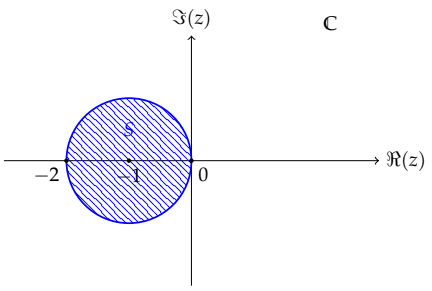
\includegraphics[height=0.6\textheight, width=0.6\textwidth, keepaspectratio]{./Images/ros_euler_10.png}
		\end{center}
	\end{figure}

\end{example}
\begin{example}[Estabilidade do Método de Euler Implícito]
	Para o método implícito, temos
	\[
		\lim_{n\to \infty}U^{n} = 0 \Longleftrightarrow | 1-z | > 1,
	\]
	onde \(z = h\lambda , \lambda \in \mathbb{C}\).

	Logo, em contraste ao explícito, a região de estabilidade do método de Euler implícito é a região exterior ao disco de centro em 1 e raio 1:
	\begin{figure}[H]
		\begin{center}
			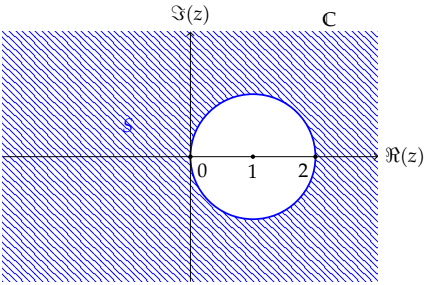
\includegraphics[height=0.6\textheight, width=0.6\textwidth, keepaspectratio]{./Images/ros_ieuler_10.png}
		\end{center}
	\end{figure}
\end{example}
\begin{example}[Estabilidade do Método do Trapézio]
	Sendo \(\lambda \in \mathbb{C}\), temos
	\[
		\lim_{n\to \infty}U^{n} = 0 \Longleftrightarrow \biggl\vert \frac{1+\frac{z}{2}}{1-\frac{z}{2}} \biggr\vert < 1,
	\]
	que acontece apenas quando \(\mathrm{Re}(z) < 0\).

	Desse modo, a região de estabilidade do método do trapézio é todo o lado esquerdo do plano complexo:
	\begin{figure}[H]
		\begin{center}
			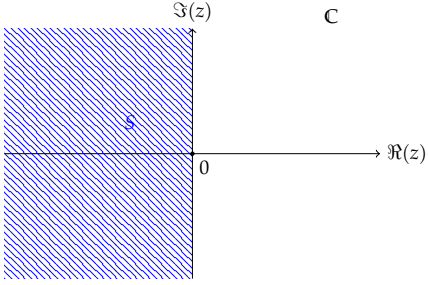
\includegraphics[height=0.6\textheight, width=0.6\textwidth, keepaspectratio]{./Images/ros_trapezoidal_10.png}
		\end{center}
	\end{figure}
\end{example}

Considere agora um sistema linear de EDO's dado por
\[
	\mathbf{u}'(t) = A \mathbf{u}(t), \quad \mathbf{u}(0) = \underline{\lambda} ,
\]
onde \(A\in \mathbb{R}^{m\times m}\) é constante e diagonalizável.

Como ela é diagonalizável, existem m autovetores linearmente independentes para a matriz A; denotando-os por \(\mathbf{v}^{i}\), eles são associados a m autovalores \(\lambda_{i}\in \mathbb{C}\), tal que
\[
	A \mathbf{v}^{i} = \lambda_{i}\mathbf{v}^{i}, \quad i=1, \dotsc , m.
\]
Seja, também, \(R = [\mathbf{v}^{1}, \mathbf{v}^{2}, \dotsc , \mathbf{v}^{m}]\) a matriz cujas colunas são os autovetores \(\mathbf{v}^{i}\), e \(\Lambda \) uma matriz diagonal com os autovalores \(\lambda_{i}\), de forma que a diagonalizabilidade de A permite escrevermos
\[
	A = R \Lambda R^{-1}
\]
e, assim,
\[
	\Lambda  = R^{-1}AR.
\]

Portanto, faz sentido definir a transformação linear
\[
	\mathbf{v}(t) = R^{-1}\mathbf{u}(t) \Rightarrow \mathbf{v}'(t)=R^{-1}\mathbf{u}'(t),
\]
tal que
\begin{align*}
	            & \mathbf{u}'(t) = A \mathbf{u}(t)                    \\
	\Rightarrow & R^{-1}\mathbf{u}'(t) = R^{-1}ARR^{-1} \mathbf{u}(t) \\
	\Rightarrow & \mathbf{v}'(t) = R^{-1}AR \mathbf{v}(t)             \\
	\Rightarrow & \mathbf{v}'(t) = \Lambda \mathbf{v}(t),
\end{align*}
transformando o sistema de EDO's no sistema desacoplado
\[
	v_{j}'(t) = \lambda_{j} v_{j}(t), \quad j=1, 2, \dotsc , m.
\]
\begin{def*}
	Um método geral de um passo é dito \textbf{absolutamente estável} para um sistema linear da forma
	\[
		\mathbf{u}'(t) = A \mathbf{u}(t), \quad \mathbf{u}(0) = \underline{\lambda },
	\]
	onde A é uma matriz m por m real e diagonalizável, se \(z_{j} = h\lambda_{j}\in S\) para todos os autovalores \(\lambda_{j}\) da matriz A, qualquer que seja a escolha de \(h > 0.\)

	Caso haja uma condição sobre h para que essa condição seja satisfeita, o método é dito \textbf{condicionalmente estável}. \(\square\)
\end{def*}
\end{document}
